\chapter{Specifikáció}

\section{A program célja}
A program célja tetszőleges adat tömörítése majd ezek kitömörítése információvesztés nélkül.
Ennek megvalósítására a Shanon-Fano tömörítő algoritmust
\footnote{C. E. Shannon, „A Mathematical Theory of Communication”, 1948}
\footnote{Robert M. Fano, „The Transmittion of Information”, 1949}
alkalmazza.

\section{Felhasználói interakció}
A felhasználó két üzemmódot választhat ki a program futtatásakor: kódolás vagy dekódolás. Ezeket az első parancssori argumentumban a 
'kodol' és 'dekodol' kulcsszavakkal tudja kiválasztani.
\subsection{kódolás (kodol)}
\label{sec:encode}
Kódoló üzemmódban a bemenetet (lásd \nameref{ssec:in}) a Shanon-Fano kódoló algoritmust alkalmazva írja a kimenetre (lásd \nameref{ssec:out}) a kódolt adatot.
\begin{verbatim}
    program kodol --bemenet <fájl> --kimenet <fájl>
\end{verbatim}
\subsection{dekódolás (dekodol)}
\label{sec:decode}
Dekódoló üzemmódban a bemenetet (lásd \nameref{ssec:in}) a Shanon-Fano dekódoló algoritmust alkalmazva írja a kimenetre (lásd \nameref{ssec:out}) a dekódolt adatot.
\begin{verbatim}
    program dekodol --bemenet <fájl> --kimenet <fájl>
\end{verbatim}

\newpage
\section{A program által elfogadott kapcsolók}
\label{sec:flags}
A program futása során tetszőleges futtatást befolyásoló kapcsolókat (flageket) beállíthatunk.
Ezek sorrendje tetszőlegesen választható.
\subsection{Bemenet}
\label{ssec:in}
Parancssori megnevezés: \texttt{-{}-bemenet <forrásfájl>} \\
{\it Opcionális paraméter.}\\
Ha nincs megadva, de a program egy figyelmeztető üzenet kíséretében folytatja a lefutást. \\
A fájl méretétől és tartalmától független a program lefutása. \\
Az azt követő paraméter megadja a forrásfájl elérési útvonalát. Ha nincs megadva, stdin-ról kér be új sorral lezárt szöveget.

\subsection{Kimenet}
\label{ssec:out}
Parancssori megnevezés: \texttt{-{}-kimenet <célfájl>} \\
{\it Opcionális paraméter.}\\
Ha nincs megadva, de a program egy figyelmeztető üzenet kíséretében folytatja a lefutást.\\
A fájl méretétől és tartalmától független a program lefutása. \\
Az azt követő paraméter megadja a célfájl elérési útvonalát. Ha nincs megadva, stdout-ra írja ki a program a program kimenetét.

\subsection{Kódtábla}
Parancssori megnevezés: \texttt{-{}-kodtabla} \\
{\it Opcionális paraméter.}\\
Azt szabályozza, hogy a kódtáblát kiírja-e a program a standard kimenetre.

\subsection{Statisztika}
Parancssori megnevezés: \texttt{-{}-statisztika} \\
{\it Opcionális paraméter.}\\
Azt határozza meg, hogy a program kiírjon-e további számitásokat a program hatékonyságára vonatkozólag.\\
Az alábbi számítások történnek kiírásra: \\
\begin{itemize}
    \item Tömörítés mértéke: bemenet mérete a tömörített adat méretéhez képest
    \item Kódtábal mérete: Egymástól eltérő kódok száma
    \item Kódok mérete: legrövidebb kód, leghosszabb kód, kódok átlagos mérete
    \item Fa mérete: A generált fa mérete
\end{itemize}

\subsection{Segítség}
Parancssori megnevezés: \texttt{-{}-help} \\
{\it Opcionális paraméter.}\\
A felhasználót tájékoztatja a program helyes használatáról. Ha ez a kapcsoló meg van adva, akkor a program nem ellenőrzi
a többi kötelező kapcsoló jelenlétét, kiírja a szöveget majd kódolás / dekódolás nélkül befejezi a futást.\\
Az alábbi szöveg íródik ki: \\
\begin{verbatim}    
    program [üzemmód] <...kapcsolók...>
    Üzemmód: kodol, dekodol
    Kapcsolók:
    --bemenet <forrásfájl>: Bemeneti fájl (ha üres akkor stdin)
    --kimenet <célfájl>: Bemeneti fájl (ha üres akkor stdout)
    --kodtabla <fájl>: A kódtábla fájl (kötelező)
    --statisztika: A tömörítés hatékonyságát értékelő statisztika (opcionális)
    --help: Ezt az üzenetet írja ki (opcionális)
\end{verbatim}


\section{A program kimenete}
Sikeres futtatás esetén a program a \nameref{sec:flags} pontban meghatározott viselkedés szerint működik.
Sikertelen futtatás esetén a konzolra kiíródik a probléma és egy nem nullás kilépési kóddal a program megáll. \\
A fájl ami generálódik a következőképpen épül fel:
Kódtábla karaktereinek száma: Hány darab karaktert és annak kódolását tartalmaz a kódtábla. Lehetséges értékei: 0-255 --> 1-256 \\
Illeszkedés hossza: A fájl végén hány darab 0 bit van a 8 bites fájlmentés kielégítéséhez. \\
Kódtábla, melynek minden eleme az alábbiakból épül fel:\\
\begin{itemize}
    \item Karakter: nyolc bit, melyet tömörítünk
    \item a karaktert reprezentáló kód hossza 8 biten
    \item a kód, mely nullás és eggyesek sorozata
\end{itemize}
Kódolt adat

\begin{figure}[H]
    \centerline{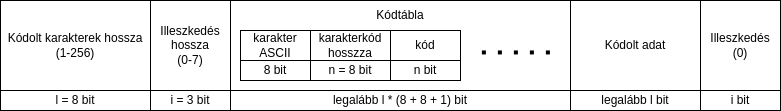
\includegraphics[width=\linewidth]{encodedfilecontents.png}}
\end{figure}